%!TEX root = ../Systementwurf.tex

\chapter{Resultierende Softwarearchitektur}\label{chap:architektur}

Die \NewsGenie Systemarchitektur ist eine klassische Client-Server Architektur, wobei es sich um einen Thin-Client
und einen Fat-Server handelt. Sämtliche Rechenaufwändige Operationen werden dementsprechend auf dem \textit{Server} ausgeführt,
während der \textit{Client} die sprachbasierte Bedienung durch den User umsetzt. Allerdings werden kleinere und ressourcenarme  Sprachverarbeitungsdienste zum Zweck einer zeitlichen Performancesteigerung ebenfalls am \textit{Client}
realisiert. Diese beinhalten die Verarbeitung von Anfragen der einfachsten Art, in erster Linie einfache Navigationsbefehle, wie das Auswählen eines von mehreren vorgeschlagenen Nachrichtenartikeln. 
Die Kommunikation mit der \textit{Google-Speech-API} findet ebenfalls auf dem \textit{Client} statt.

Die Architektur des \textit{Servers} ist in vier Komponenten geteilt. Das Kernelement für die Datenspeicherung ist 
die mit Triplen realisierte \textit{Datenbank} und der \textit{Crawler}, welcher permanent die ausgewählten Nachrichtenseiten nach neuen Artikeln durchsucht, um diese dann speichern zu lassen. Aus der vom \textit{Client} empfangenen Useranfrage und den vorhandenen Artikeln in der \textit{Datenbank} eine relevante Antwort zu generieren ist Aufgabe des \textit{Query Processors}. 
Der \textit{Server} bietet darüber hinaus ein \textit{Web Interface} an, welches es dem User oder Administrator ermöglicht Benutzereinstellungen zu verändern.

Die Architektur des \textit{Query Processors} unterteilt sich in sechs weitere Komponenten. Herzstück ist der \textit{Query Handler}.
Diese Komponente steuert den Ablauf des \textit{Query Processors} und regelt das Zusammenspiel der anderen Komponenten. 
Die erste anzusteuernde Komponente ist \textit{Natural Language Processing}, welches die Satzstruktur der Useranfrage analysiert. Darauf aufbauend ist es im \textit{Analyzer} möglich die Intention der Nutzeranfrage zu bestimmen, wie z.B. Neuigkeiten im Bereich der Technologie zu finden, oder Informationen zu einer bestimmten Person zu nennen. 
Der \textit{Searcher} kann dementsprechend agieren und eine geeignete Anfrage an die Datenbank stellen. Im Falle einer Entitätsfrage, wie das erwähnte Fragen nach dem Alter einer Person, wird die \textit{Linked Open Data}-Komponente angesteuert, andernfalls die \textit{Datenbank}.
Die Informationen der Linked Open Data können durch die \textit{Linked Open Data} Komponente schnell und effizient abgefragt werden, um dementsprechende faktuale Anfragen beantworten zu können. 
Die bis hierhin entstandenen Ergebnisse des Prozesses werden daraufhin an die \textit{Result Processing} Komponente übermittelt.
Aufgabe dieser ist es, die Ergebnisse für die Sprachausgabe am \textit{Client} vorzubereiten, also den Ausgabestring zu generieren. Dazu zählt auch die Aufgabe durch Textbausteine für eine natürlich klingende und abwechslungsreiche Sprache zu sorgen.

\section{Komponentenspezifikation}

%In diesem Abschnitt wird die aus der Analyse der Produktfunktionen (\autoref{chap:analyse}) resultierende Komponentenstruktur zunächst überblickartig durch ein Komponentendiagramm beschrieben. Die Bezeichnungen und Anzahl der Komponenten
%muss natürlich konsistent sein mit der in \autoref{chap:analyse}!

%Die einzelnen Komponenten werden anschließend kurz beschrieben.

Die aus Abschnitt \ref{chap:analyse} resultierende Komponentenarchitektur ist in Abb.~\ref{fig:Komponenten} in Form eines Komponentendiagramms abgebildet. Die Komponente \textit{Query Processor} wird außerdem in Abb.~\ref{fig:Komponenten_QP} in ihre Unterkomponenten aufgeschlüsselt.

\begin{figure}
\centering
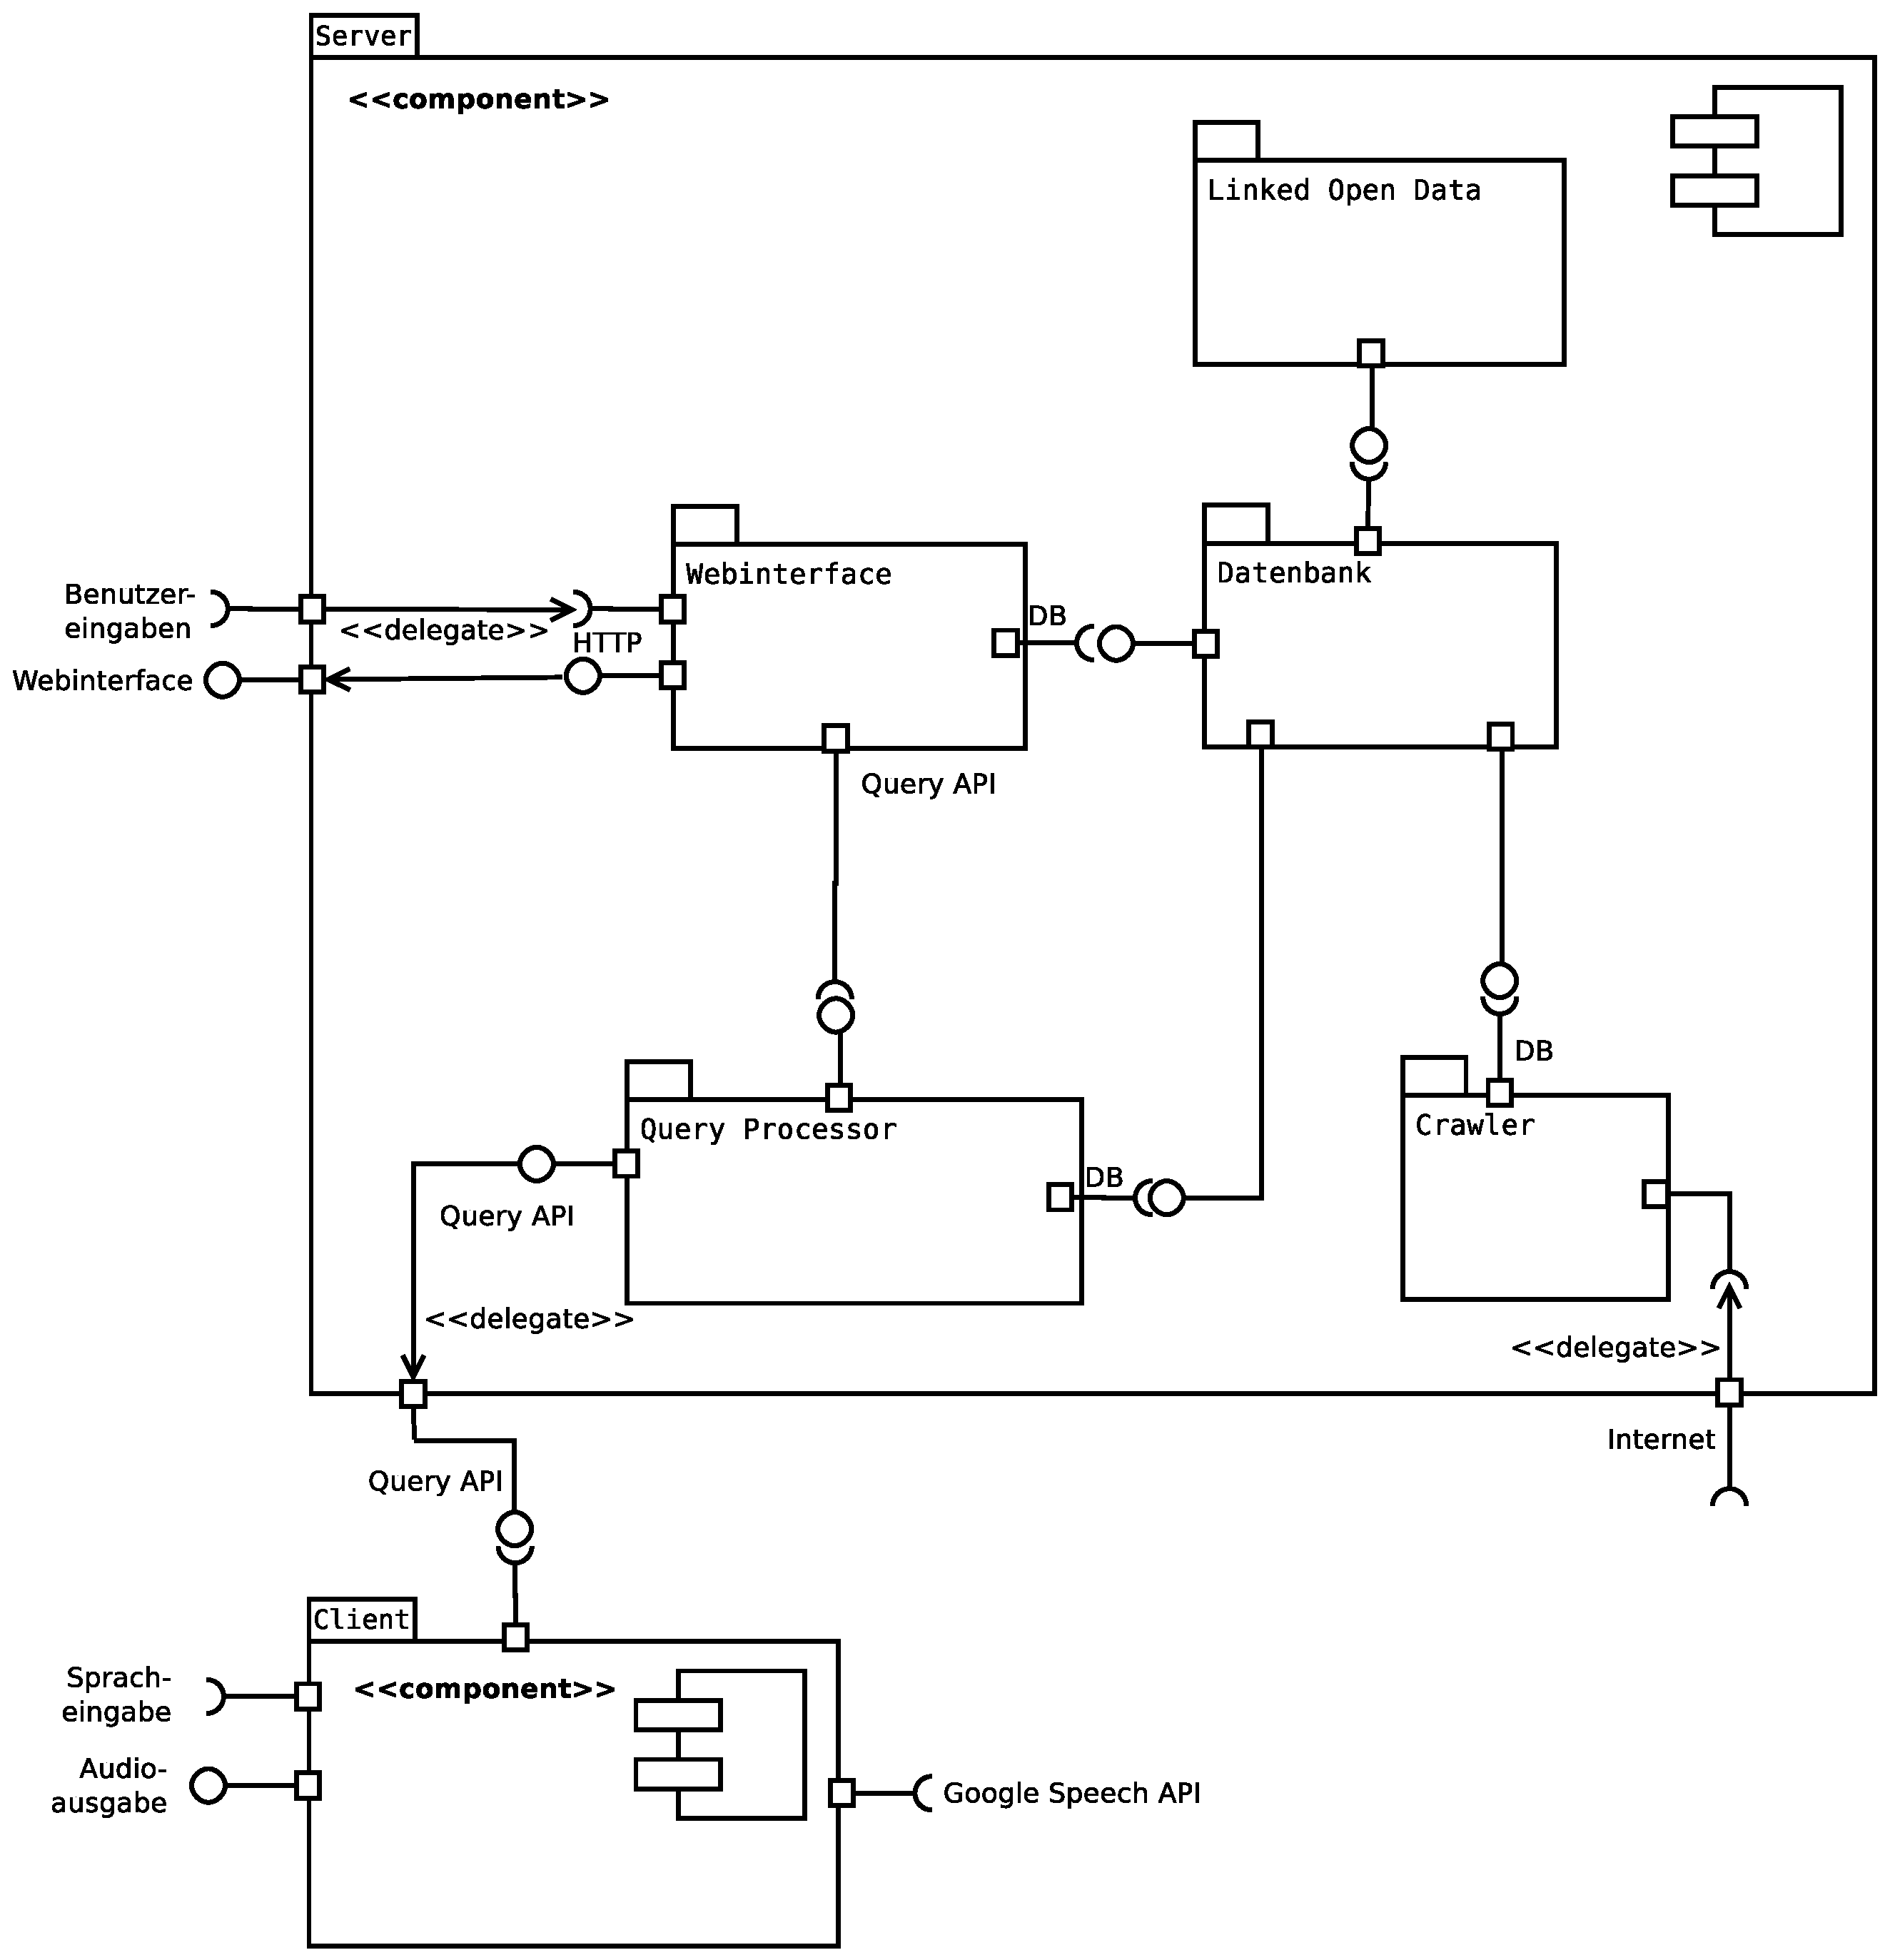
\includegraphics[width=1\linewidth]{Systementwurf/05_implementierungsentwurf/komponenten}
\caption{\textit{\NewsGenie Komponentendiagramm}}
\label{fig:Komponenten}
\end{figure}

\begin{figure}
\centering
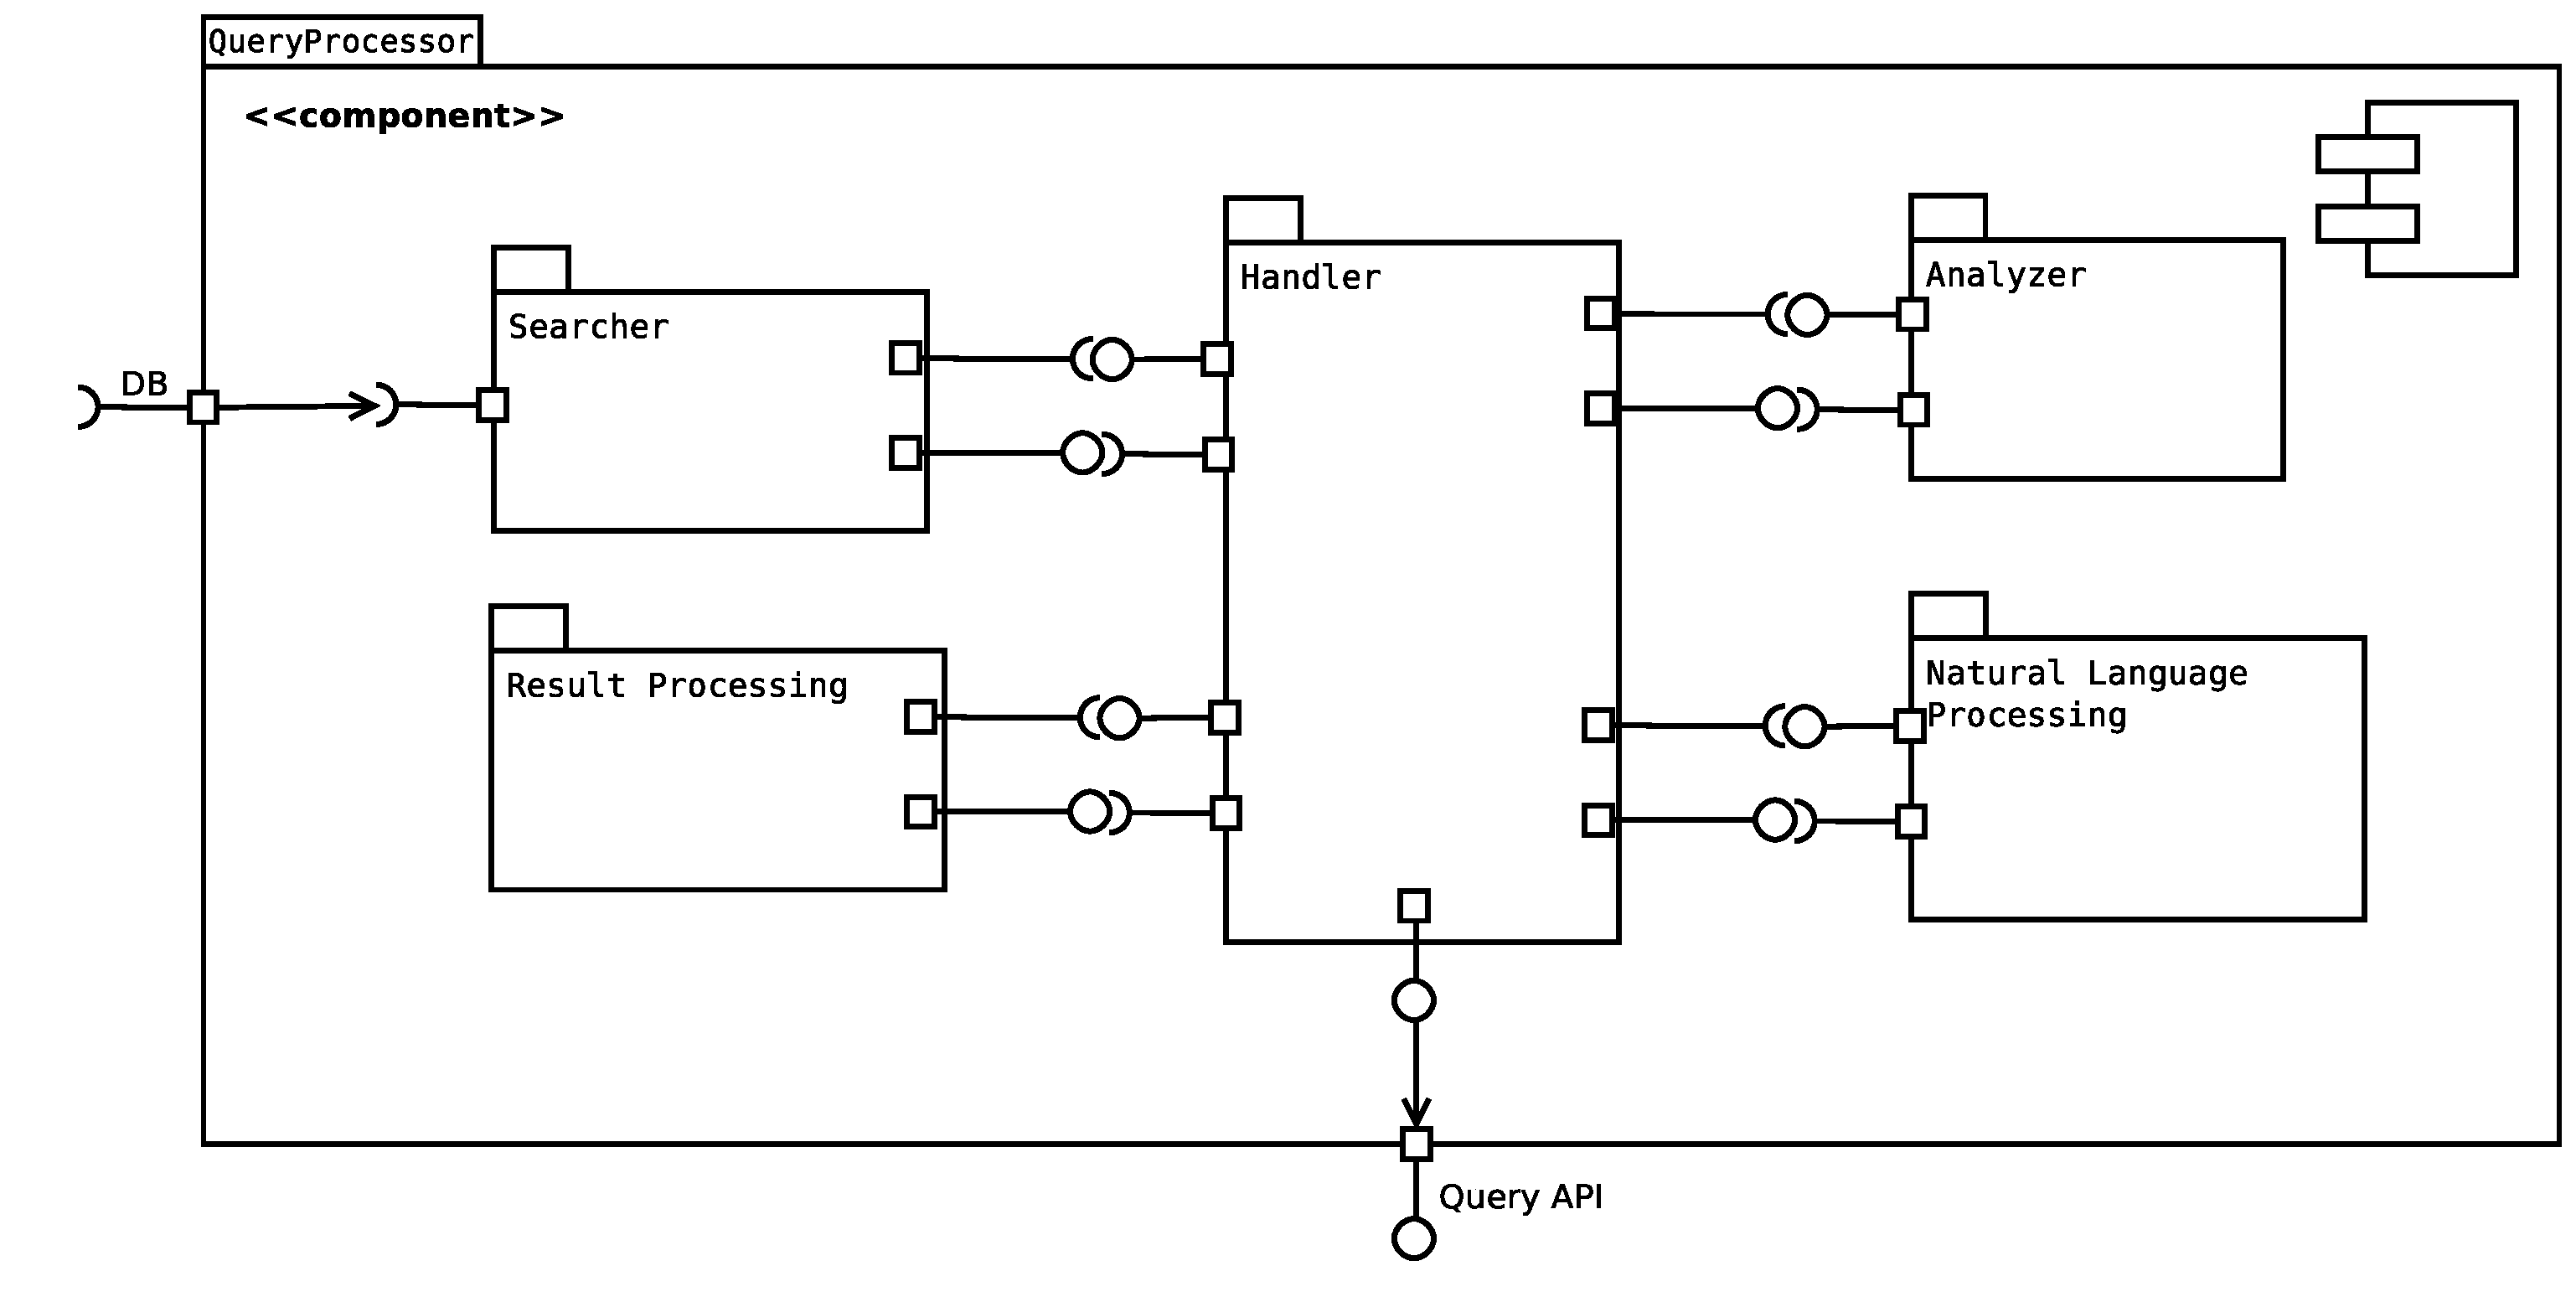
\includegraphics[width=1\textheight, angle=90]{Systementwurf/05_implementierungsentwurf/paket-queryprocessor}
\caption{\textit{\NewsGenie Komponentendiagramm - Query Processor}}
\label{fig:Komponenten_QP}
\end{figure}

\begin{component}{10}{Client}
Auf dem \textit{Client} werden die Hauptfunktionen der Sprach Ein- und Ausgabe realisiert. Der \textit{Client} ist somit die Hauptschnittstelle des Benutzers. Der Zugriff auf die \textit{Google Speech API} wird auf dem \textit{Client} realisiert. 
Die Komponente ist zusätzlich dazu in der Lage, auf simple Navigationsbefehle zu reagieren, ohne den \textit{Server} 
kontaktieren zu müssen.
\end{component}

\begin{component}{20}{Webinterface}
Das \textit{Web Interface} ist die zweite Schnittstelle für den Benutzer. Es stellt Konfigurations- und 
Administrationsfunktionen zur Verfügung, wie Nutzerregistrierung, Passwortmanagement, das Abonnement-Management
der Nachrichtenfeeds oder auch das Löschen von Nutzern.
\end{component}

\begin{component}{30}{Datenbank}
Realisiert die Speicherung der relevanten Daten über die User und die Nachrichtenartikel.
Die Speicherstruktur ist mit Tripeln implementiert.
\end{component}

\begin{component}{35}{Linked Open Data}
Komponente für den Zugriff auf die Linked Open Data. Sie liefert Informationen zu bestimmten
Entitätsfragen nach Personen oder Orten.
\end{component}

\begin{component}{40}{Crawler}
Der \textit{Crawler} liefert die Daten für die \textit{Datenbank}, indem er das Internet nach Nachrichtenartikeln
durchsucht, welche anschliessend gespeichert werden.
\end{component}

\begin{component}{50}{Query Processor}
Der \textit{Query Processor} verarbeitet die am \textit{Client}/\textit{Web Interface} gestellten Anfragen um die Intention
des Users zu erkennen und dementsprechend Anfragen an die \textit{Datenbank} zu stellen. Die Ergebnisse
werden an den \textit{Client} zurück gegeben.
Die Komponente besteht aus den Unterkomponenten \textit{Handler}, \textit{Natural Language Processing}, \textit{Analyzer}, \textit{Searcher}, \textit{Linked Open Data}, und \textit{Result-Processing}.
\end{component}

\begin{component}{60}{Handler}
Der \textit{Handler} steuert durch Aufrufe der anderen Komponenten den Ablauf im Query Processor. Sie ist die Komponente die von aussen angesteuert wird. 
\end{component}

\begin{component}{70}{Natural Language Processing}
Die als String eingehenden Anfragen werden auf ihre Satzstruktur analysiert. Es werden Subjekt, Objekt und Prädikat erkannt.
Darüber hinaus wird der Satz als Baumstruktur abgespeichert, was es ermöglicht Nebensätze und Hauptsätze zu erkennen. 
\end{component}

\begin{component}{80}{Analyzer}
Aufbauend auf \textit{Natural Language Processing} kann die Anfrage in dieser Komponente tiefer gehend analysiert werden. Sie bestimmt den Fragetyp, d.h. Entitätsfrage oder Nachrichtenanfrage, und kann somit die Intention des Users analysieren. 
\end{component}

\begin{component}{90}{Searcher}
Aufbauend auf den \textit{Analyzer} kann der \textit{Searcher} Datenbankanfragen stellen, um die passenden Ergebnisse zu bekommen.
Bei Entitätsfragen wird \textit{Linked Open Data} angesteuert, welche mit Daten aus der Linked Open Data antworten kann. 
\end{component}

\begin{component}{100}{Result Processing}
Im \textit{Result Processing} werden die Ergebnisse als String aufbereitet. Dabei werden variable Textbausteine verwendet um eine möglichst natürliche und flüssige Sprachausgabe zu gewährleisten.
\end{component}


\section{Schnittstellenspezifikation}

%Im Folgenden werden die einzelnen Schnittstellen der Komponenten aus der
%Komponentenspezifikation näher erläutert, d.h. die von Ihnen zur Verfügung
%gestellten Operationen werden dokumentiert. Die Tabelle ist dabei um so viele
%Zeilen zu erweitern, wie es Schnittstellen im Komponentendiagramm gibt. In der
%innen liegenden Aufteilung ist für jede Operation einer Schnittstelle eine
%Zeile einzufügen.  Reine Set- und Get-Aufrufe brauchen nicht aufgeführt zu
%werden (sollten auch möglichst nicht komponentenübergreifend auftauchen).

\textbf{Hinweis:}
Durch die Verwendung des Akka-Frameworks für die Komponenteninteraktion zwischen
Client, Server, Datenbank, Crawler und Webinterface werden, statt einzelne
Nachrichten, Objekte verschickt.
Daher sind bei Kommunikationen zwischen diesen Komponenten die Operationen als
ins Netzwerk angebotene Objekte zu betrachten.
Alle anderen Komponentenkommunikationen sind als Funktionsaufrufe aus den fünf
oben genannten Komponenten zu sehen.

\begin{interface}{10}{Client Schnittstelle}
\begin{tabular}[ht]{|p{5cm}|p{9cm}|}
\hline
Operation & Beschreibung\\
\hline
ClientQuery()  & Der Client sendet die Suchanfrage an den Handler,
welcher die Verarbeitung koordiniert.\\
\hline
\end{tabular}
\end{interface}

\begin{interface}{20}{Webinterface Schnittstelle}
\begin{tabular}{|p{5cm}|p{9cm}|}
\hline
Operation & Beschreibung\\
\hline
ClientQuery() & Das Webinterface sendet die Suchanfrage an den Handler,
welcher die Verarbeitung koordiniert.\\
\hline
RegisterRequest() & Die Anfrage einer Registrierung an den Server\\
\hline
WebLoginRequest() & Die Anfrage eines Logins an den Server\\
\hline
UserFeedsRequest() & Die Anfrage, die abbonierten Feeds eines Nutzers zu
bekommen.\\
\hline
AddFeedRequest() & Die Anfrage, einen Feed zu den abbonierten Feeds hinzuzufügen\\
\hline
RemoveFeedRequest() & Die Anfrage, einen Feed von den abbonierten Feeds zu
löschen\\
\hline
ChangePasswordRequest() & Die Anfrage, das Passwort zu ändern\\
\hline
RecoverPasswordRequest() & Die Anfrage, das Passwort wiederherzustellen\\
\hline
UserListRequest() & Die Anfrage, alle Nutzer zu bekommen\\
\hline
DeleteUserRequest() & Die Anfrage, einen User zu löschen\\
\hline
ClientQuery() & Eine Anfrage an das System stellen\\
\hline
\end{tabular}
\end{interface}

\begin{interface}{30}{Datenbank Schnittstelle}
\setlength{\LTpre}{-0,45cm}
\begin{longtable}[l]{|p{5cm}|p{9cm}|}

\hline
Operation & Beschreibung\\
\hline
SearchAnswer() & Die SearchAnswer wird zurück an den Searcher geschickt und
beinhaltet die Suchantwort\\
\hline
ClientLoginAnswer() & Die CLientLoginAnswer wird zurück an den Client geschickt
und beinhaltet den Status, ob der User seine Logindaten korrekt eingegeben hat\\
\hline
RegisterAnswer() & Die RegisterAnswer wird zurück an das Webinterface geschickt
und beinhaltet den Status, ob der User seine Registrierung erfolgreich
abgeschlossen hat\\
\hline
WebLoginAnswer() & Die RegisterAnswer wird zurück an das Webinterface geschickt
und beinhaltet den Status, ob der User seine Logindaten korrekt eingegeben hat\\
\hline
UserFeedsAnswer() & Die UserFeedAnswer wird zurück an das Webinterface geschickt
und beinhaltet eine Liste mit allen abbonierten Feeds des Nutzers\\
\hline
AddFeedAnswer() & Die AddFeedAnswer wird zurück an das Webinterface geschickt
und beinhaltet den Status, ob das Hinzufügen bzw. Löschen eines Feeds für den
Nutzer erfolgreich war\\
\hline
ChangePasswordAnswer() & Die ChangePasswordAnswer wird zurück an das Webinterface geschickt
und beinhaltet den Status, ob das Ändern des Passworts für den
Nutzer erfolgreich war\\
\hline
RecoverPasswordAnswer() & Die RecoverPasswordAnswer wird zurück an das Webinterface geschickt
und beinhaltet den Status, ob das Zurücksetzen des Passworts für den
Nutzer erfolgreich war\\
\hline
UserListAnswer() & Die UserFeedAnswer wird zurück an das Webinterface geschickt
und beinhaltet eine Liste mit allen Nutzern\\
\hline
DeleteUserAnswer() & Die DeleteUserAnswer wird zurück an das Webinterface geschickt
und beinhaltet den Status, ob das Löschen eines Nutzers erfolgreich war\\
\hline
FactAnswer() & Die FactAnswer wird von Linked Open Data zurück an den Searcher
geschickt und beinhaltet die Link Open Data Antwort\\
\hline
UpdateArticleAnswer() & Die UpdateFeedAnswer wird zurück an den Crawler
geschickt und beinhaltet den Status, ob das Hinzufügen erfolgreich war\\
\hline
\end{longtable}
\end{interface}

\begin{interface}{40}{Crawler Schnittstelle}
\begin{tabular}[ht]{|p{4cm}|p{10cm}|}
\hline
Operation & Beschreibung\\
\hline
CrawlerAnswer() & Der Crawler sendet eine Liste von Artikeln, welche von
der Datenbank hinzugefügt werden sollen\\
\hline
\end{tabular}
\end{interface}

\begin{interface}{50}{Query Processor Handler Schnittstelle}
\begin{tabular}[ht]{|p{4cm}|p{10cm}|}
\hline
Operation & Beschreibung\\
\hline
ClientAnswer() & Die ClientAnswer wird zurück an den Managment Handler
geschickt und beinhaltet die Antwort auf die Nutzeranfrage\\
\hline
\end{tabular}
\end{interface}

\begin{interface}{60}{Managment Handler Schnittstelle}
\begin{tabular}[ht]{|p{4cm}|p{10cm}|}
\hline
Operation & Beschreibung\\
\hline
ClientQuery()  & Query Processor bekommt vom Handler die Suchanfrage und
koordiniert die Verarbeitung dieser.\\
\hline
ClientAnswer() & ClientAnswer wird vom QueryProcessor an den Client
weitergeleitet.\\
\hline
\end{tabular}
\end{interface}

\begin{interface}{70}{Natural Language Processing Schnittstelle}
\begin{tabular}[ht]{|p{4cm}|p{10cm}|}
\hline
Operation & Beschreibung\\
\hline
analyse() & Verarbeitet den übergebenen Text und gibt eine Liste der Tokens an
den Query Processor Handler\\
\hline
 \end{tabular}
\end{interface}

\begin{interface}{80}{Analyzer Schnittstelle}
\begin{tabular}[ht]{|p{4cm}|p{10cm}|}
\hline
Operation & Beschreibung\\
\hline
analyse() & Verarbeitet die übergebene Liste von Tokens und gibt alles Nötige
für die Datenbanksuche an den Query Processor Handler\\
\hline
 \end{tabular}
\end{interface}

\begin{interface}{90}{Searcher Schnittstelle}
\begin{tabular}[ht]{|p{4cm}|p{10cm}|}
\hline
Operation & Beschreibung\\
\hline
SearchRequest() & Ein SimpleSearchRequest wird an die Datenbank
geschickt mit allen nötigen Informationen für die Suche\\
\hline
search() & Sucht mithilfe des SimpleSearchRequest in der Datenbank\\
\hline
 \end{tabular}
\end{interface}

\begin{interface}{100}{Result Processing Schnittstelle}
\begin{tabular}[ht]{|p{4cm}|p{10cm}|}
\hline
Operation & Beschreibung\\
\hline
makeClientAnswer() & Eine ClientAnswer wird erstellt und an den Query Processor
Handler zurückgegeben\\
\hline
 \end{tabular}
\end{interface}

\begin{interface}{110}{Linked Open Data Schnittstelle}
\begin{tabular}[ht]{|p{4cm}|p{10cm}|}
\hline
Operation & Beschreibung\\
\hline
searchfor() & Eine FactAnswer wird erstellt und an die Datenbank zurückgegeben\\
\hline
 \end{tabular}
\end{interface}



\section{Protokolle für die Benutzung der Komponenten}

Speziell der \textit{Client} ist auch in anderen Projekten sinnvoll nutzbar.
Er realisiert eine Komponente mit sprachbasiertem In- und Output, welche auch in einem gänzlich anderen Kontext genutzt werden kann.
Der \textit{Server} dagegen erfordert lediglich eine User Input-Komponente, wie z.B. den \textit{Client} um zu funktionieren. 
Ein alternatives Szenario wäre somit nur der Austausch der Nutzerschnittstelle, wobei die Kernfunktionen des Projektes gleich blieben.
Es ist allerdings denkbar, Unterkomponenten des \textit{Servers} in anderen Zusammenhängen zu verwenden.
Das Web-Crawling nach News durch den \textit{Crawler} ließe sich z.B. auch in anderen Projekten verwenden.
Der \textit{Query Processor} ist zu stark spezialisiert auf das gegebene Aufgabenfeld als dass er wirklich sinnvoll generisch in anderen Projekten genutzt werden könnte. Die Unterkomponenten \textit{Natural Language Processing} und \textit{Linked Open Data} könnten
theoretisch in andere Bereiche übernommen werden, es würde sich aber auf Grund des geringen Programmieraufwandes kaum lohnen.
Solche Klassen würde man spezialisiert auf das entsprechende Aufgabenfeld eines Projektes neu schreiben.

Der \textit{Client} und der \textit{Crawler} funktionieren als eigenständige Subsysteme und sind in Abb.~\ref{fig:client_chart} und Abb.~\ref{fig:crawler_chart} als Statecharts abgebildet.

\begin{figure}
\centering
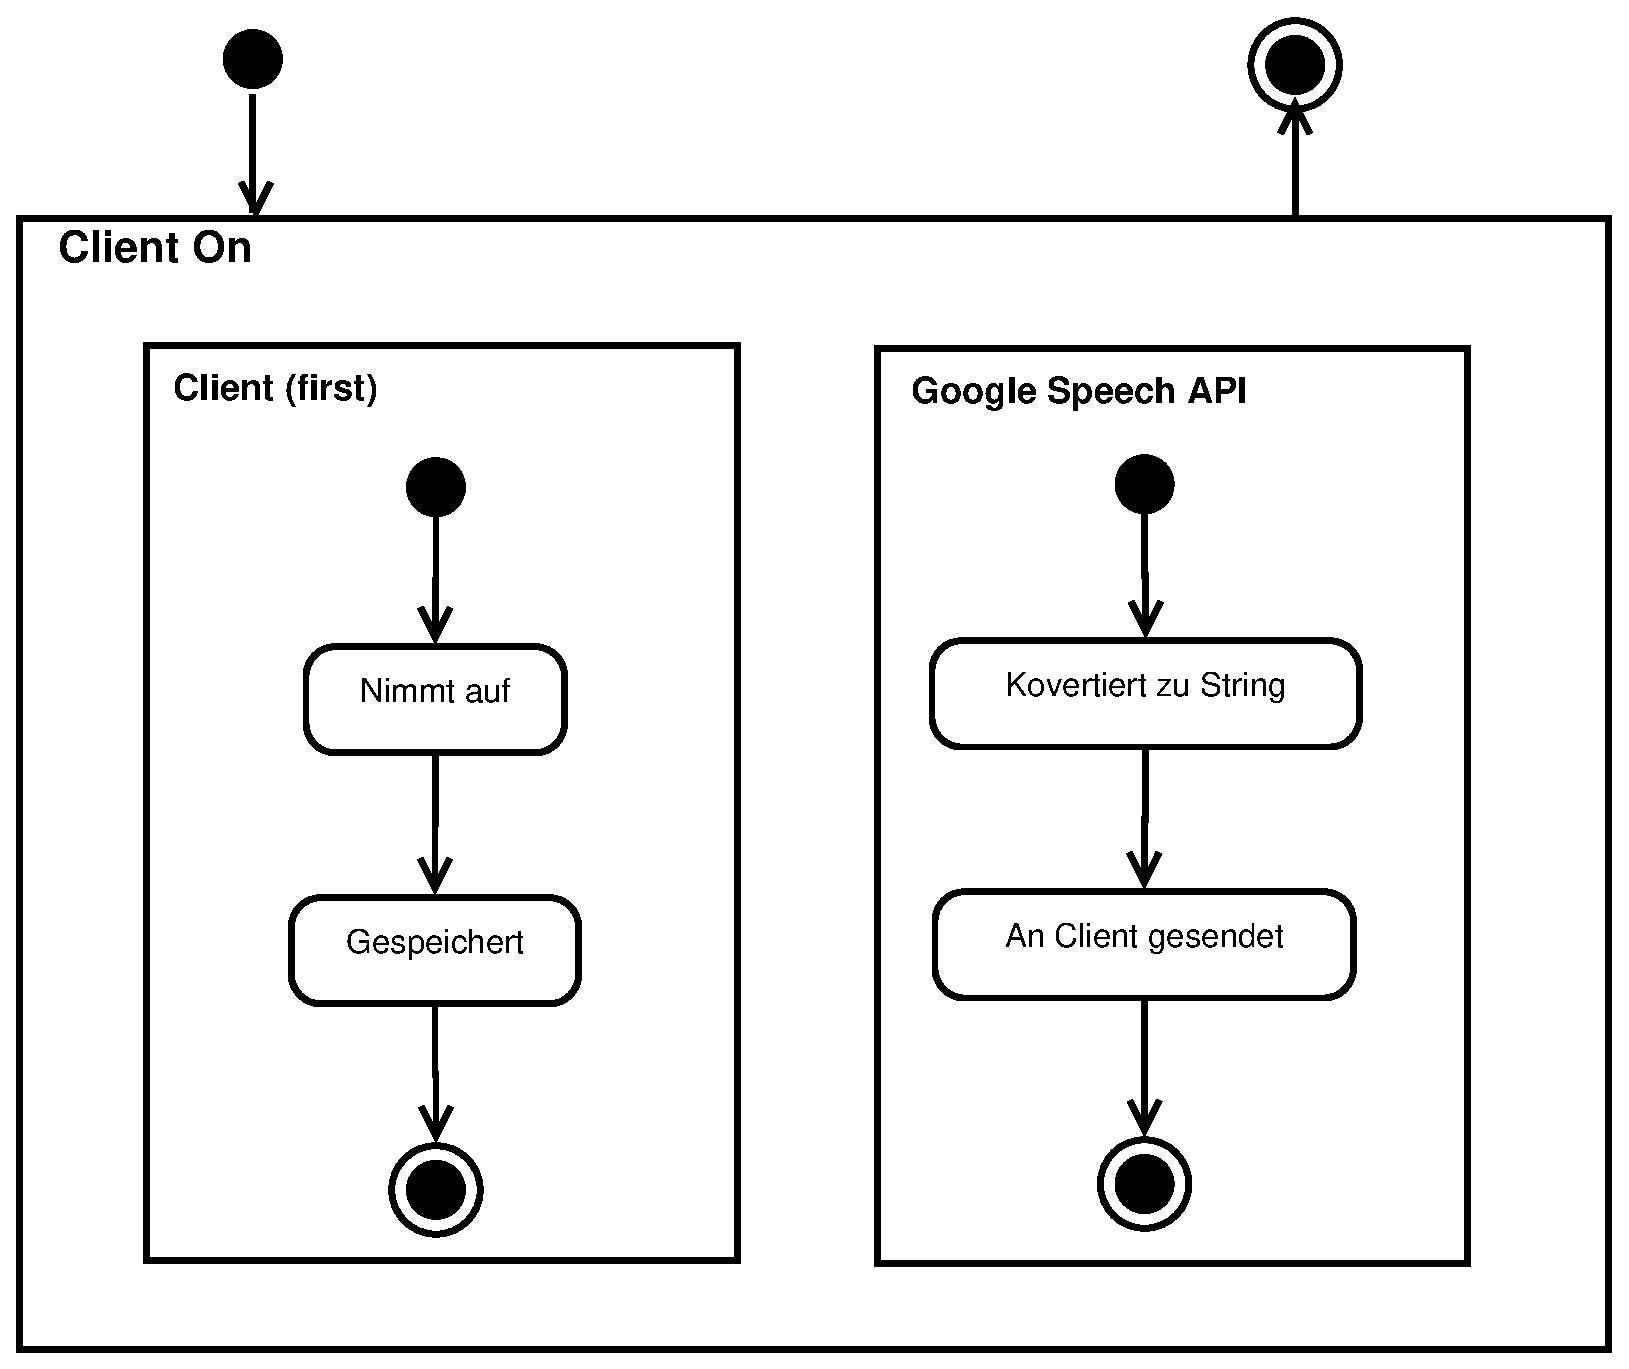
\includegraphics[width=.7\textwidth]{figures/client_chart.eps}
\caption{\textit{State Chart: Client}}
\label{fig:client_chart}
\end{figure}

\begin{figure}
\centering
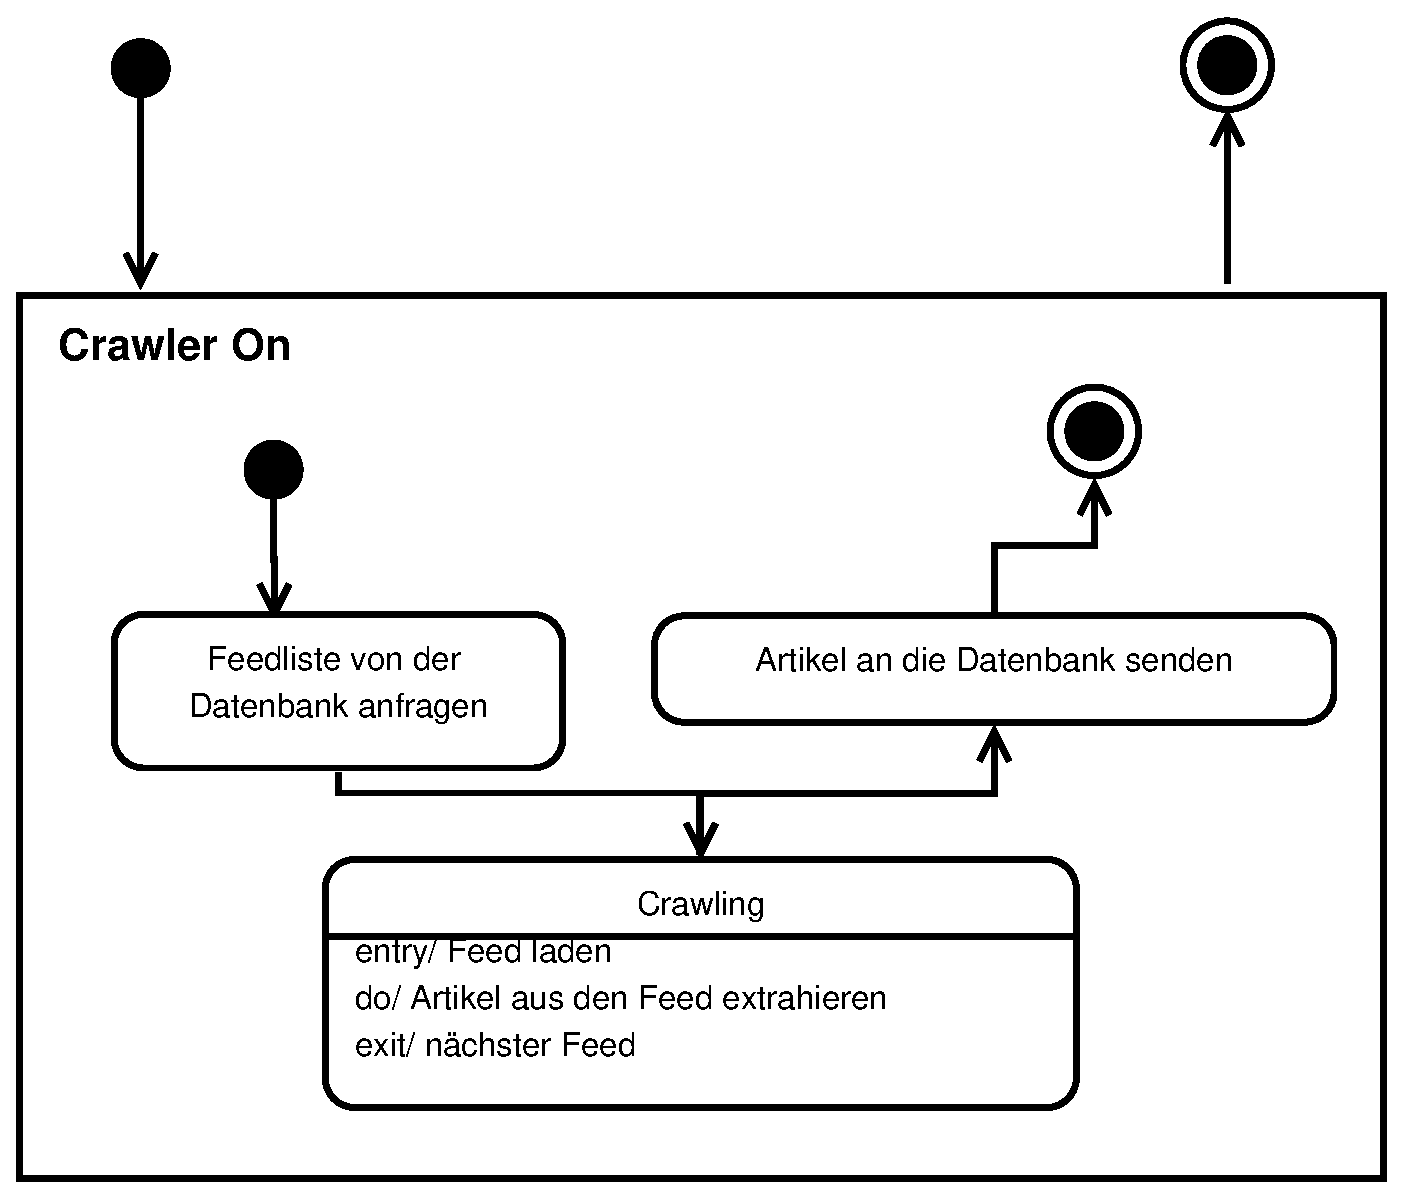
\includegraphics[width=0.7\textwidth]{figures/crawler_chart.eps}
\caption{\textit{State Chart: Crawler}}
\label{fig:crawler_chart}
\end{figure}


